\documentclass[10pt,a4paper]{article}
%\special{papersize=297mm,210mm}
\usepackage[landscape,twocolumn,margin={2cm,2cm}]{geometry}
\setlength{\columnsep}{16mm}

\usepackage[utf8]{inputenc}
\usepackage[T1]{fontenc}
%\usepackage{PTSans}
\usepackage{tgtermes} %times
% \usepackage[scaled]{uarial}
\usepackage{sectsty} %change font on headings
\allsectionsfont{\sffamily}

\usepackage{multirow}
\usepackage[hidelinks]{hyperref}
\usepackage{enumitem}
\usepackage{graphicx}
\usepackage{pdfpages}
\usepackage{rotating}
\usepackage{adjustbox}
\usepackage{epstopdf}

\title{\bf\sffamily\fontsize{18}{18}\selectfont{
Project Description\\ ETSN15 Requirements Engineering\\http://cs.lth.se/krav
}}
\author{\bf\sffamily\fontsize{12}{12}\selectfont{Björn Regnell, Elizabeth Bjarnason, Johan Linåker}}
\date{\bf\sffamily\fontsize{10}{10}\selectfont{Study period: 2020-VT1, Revision date: \today}}
\begin{document}

\maketitle
\vspace{-1cm}

\section{Objectives}
The main goals of the project from a course perspective are to:
\begin{enumerate}[noitemsep]
\item connect theory to practice,
\item give a concrete experience of practical requirements engineering,
\item promote student motivation through real stakeholders, and
\item provide a group-learning setting that is focused on realistic problems.
\end{enumerate}


\section{Context and roles}
% 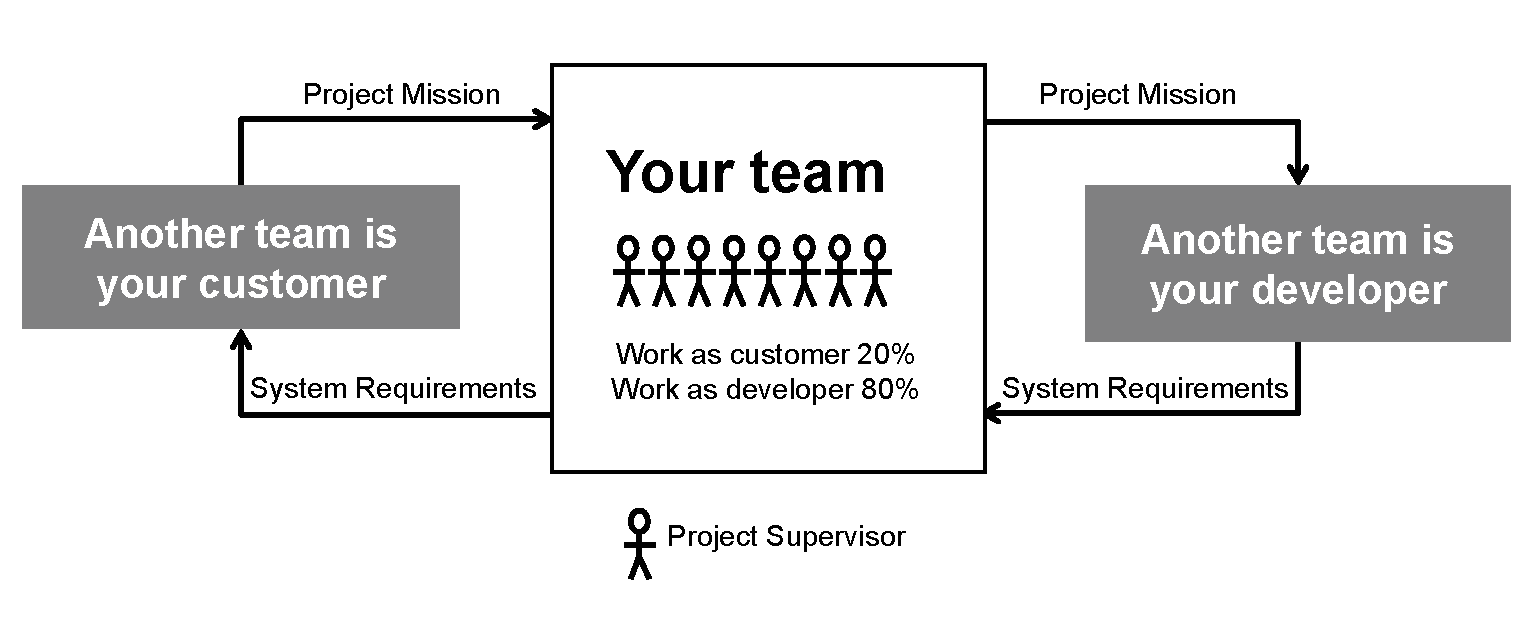
\includegraphics[scale=0.45]{fig/project-roles.eps}
% %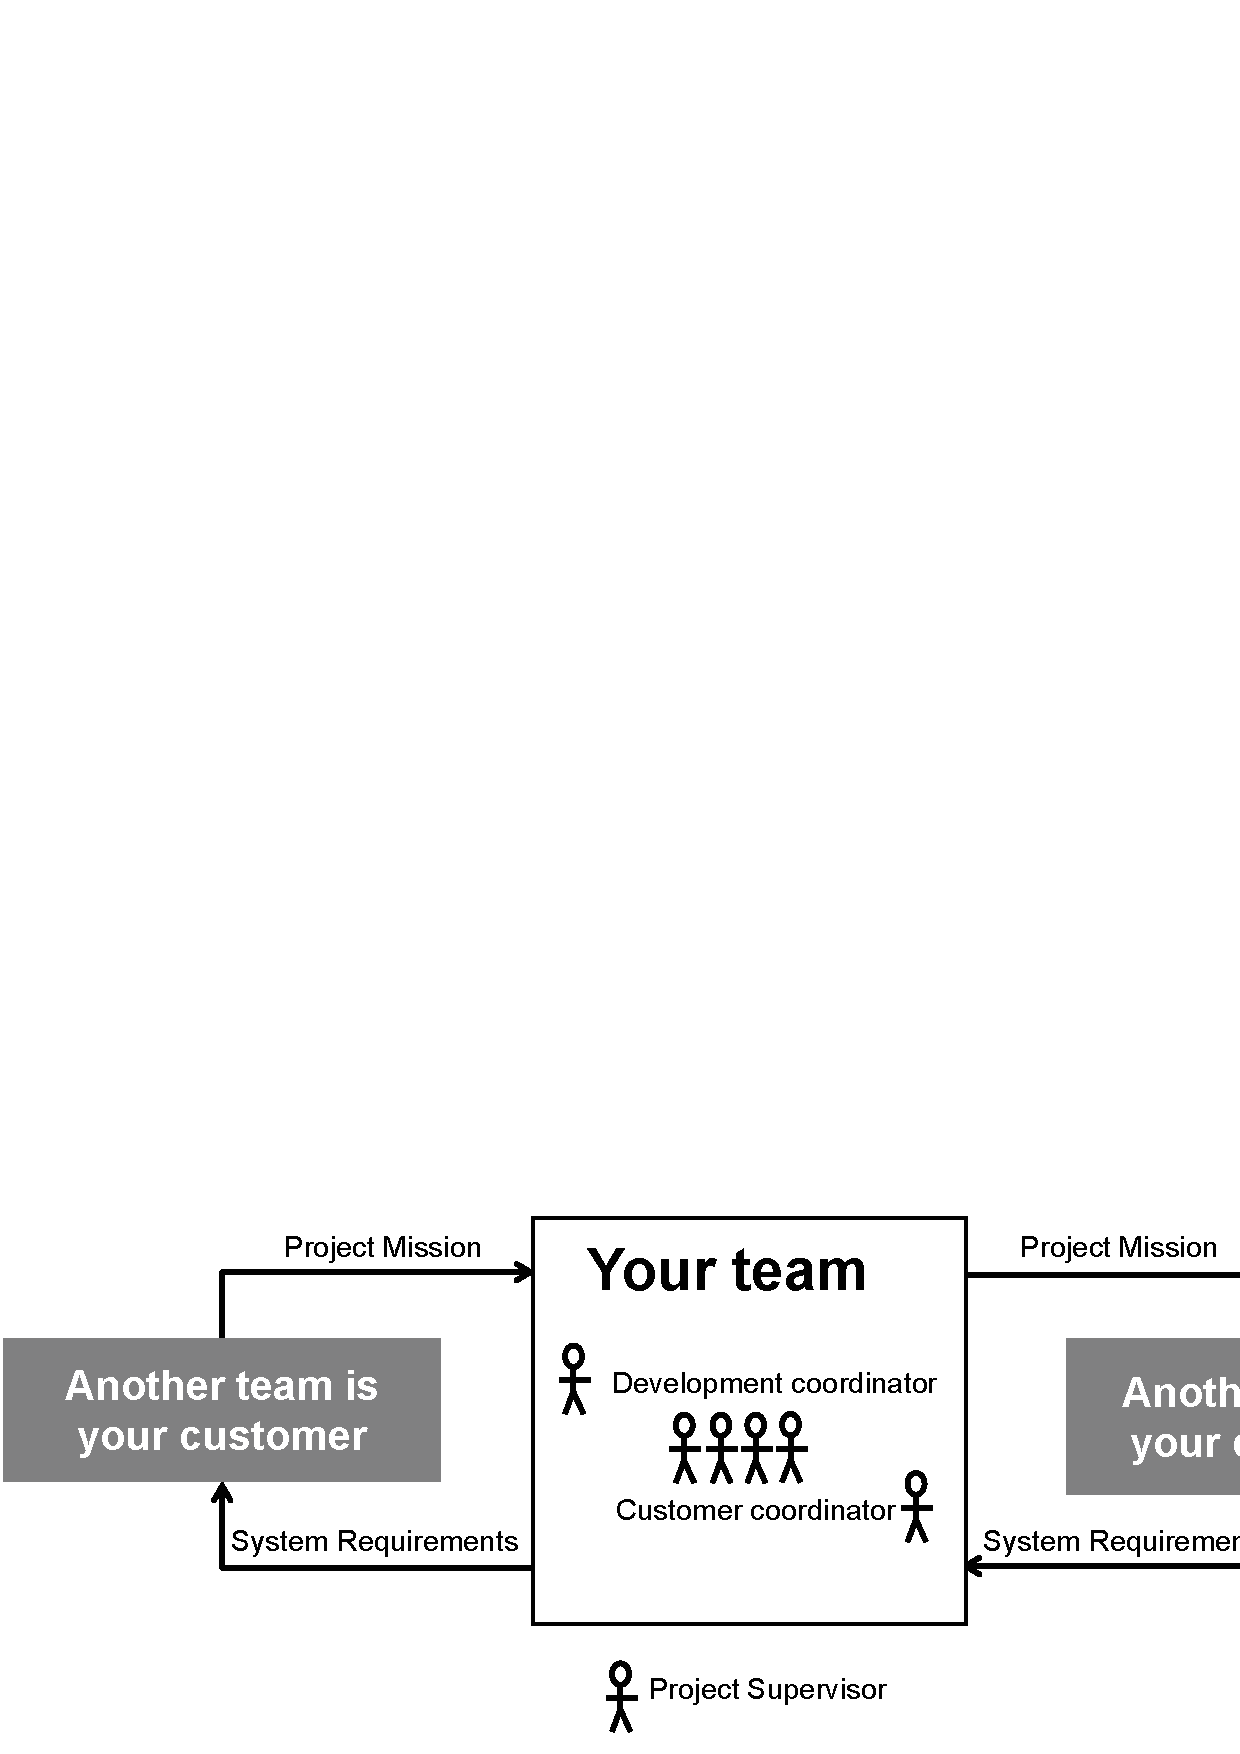
\includepdf[pages={1}]{fig/test2}
% \begin{figure}[h]
% \centering%trim = 1cm 1cm 2cm 1cm,clip,
% \vskip-1.5cm
% \hskip-2.9cm
% %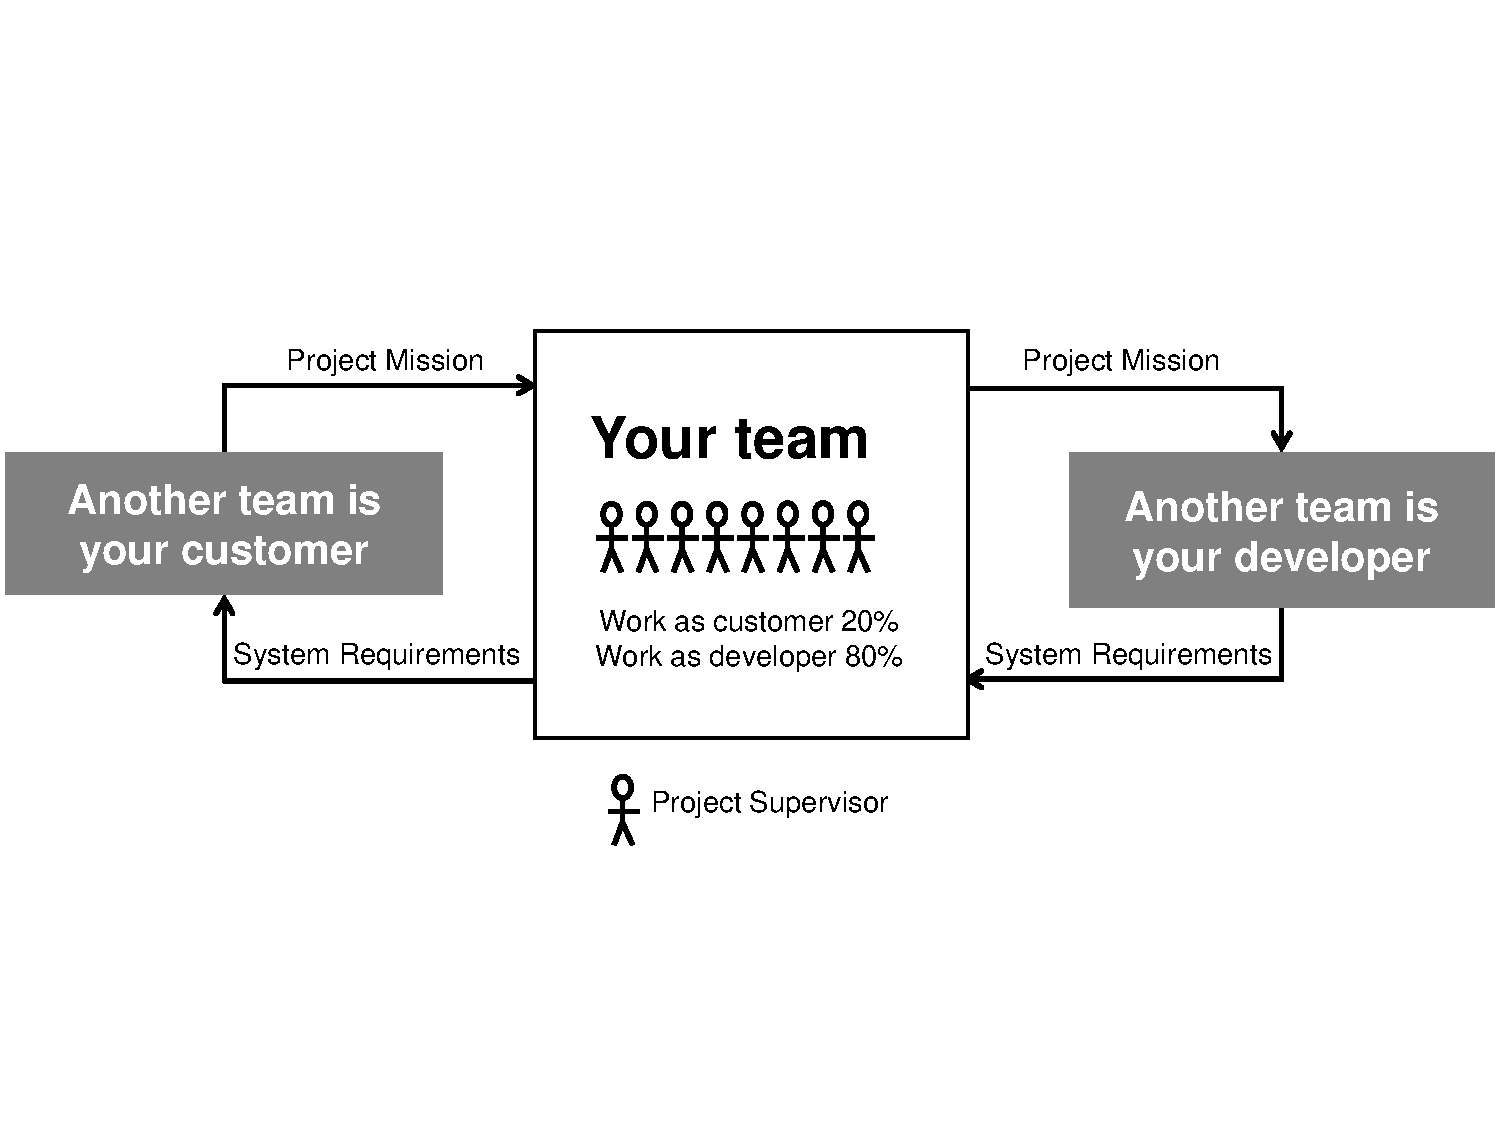
\includegraphics[trim = 5cm 6cm 1.5cm 10cm,clip,width=1.7cm]{fig/project-roles.pdf}
% \vskip0.7cm
% \end{figure}

\noindent Each project team will act as an \textit{under-consultant} to a startup company and support them with requirements engineering for their product idea. The startup companies will act as \textit{product owners} and are responsible for conveying their vision of their product idea. They will provide a Project Mission upon which the project team is to develop a system model including requirements of different types at appropriate abstraction levels. The product owners will support the project team on request, but the project team is to act independently with the Requirements Engineering process throughout the project. The product owner is to be seen as a stakeholder among many during the Requirements Engineering process.
\newline

\noindent The project team consists of 5-7 members and these managers should be appointed among team members:

\begin{description}[noitemsep]
\item[P3RM] Project, Process, Prioritization, \& Release Manager (1 pers)
\item[SPOC] Stakeholder \& Product Owner Communication (1 pers)
\item[TDEVM] Tools, Documents, Experiences \& Version Manager (1-2 pers)
\item[EPM] Elicitation \& Prototyping Manager (1-2 pers)
\item[QRM] Quality Requirements Manager (1 pers)
\item[DRVM] Data Requirements \& Validation Manager (1 pers)
\end{description}

\noindent The manager roles imply management, planning, and coordination responsibilities, but managers should not do all the work: {\it all members should contribute in all parts!}

\section{Project selection process}
\noindent The project teams will select their product idea at the second lecture in course week 1.
\newline

\noindent\textbf{Preparations:}
\begin{enumerate}[noitemsep]
  \item Read through all Projet Missions from the startup companies.
\end{enumerate}
\noindent\textbf{At lecture:}
\begin{enumerate}[noitemsep]
  \item Each product idea will be pitched by the respective startup companies
  \item Based on random order, the project teams will select the product idea that they wish to work with.
  \item The project teams and startup companies exchange contact details and agree on a first meeting.
\end{enumerate}

\section{General project rules}
\begin{enumerate}[noitemsep]
\item The project comprises 80 hours per person.
\item The total effort should be evenly distributed among participants.
\item In weeks W2, W4, and W6 a meeting should be scheduled with the project supervisor, where the project team reports on status, challenges and plans.
\end{enumerate}

\section{Project deliverables}
\begin{tabular}{l |l p{5cm}  l}
{\it Phase} & {\it Deliverables} & {\it Deadline} \\
\hline
Planning & Project Mission v2& Week 2: Thursday 09:00\\
Iteration 1 & Release R1 & Week 4: Monday 09:00 \\
Iteration 2 & Release R2  & Week 6: Monday 09:00\\
   & Validation Checklist & Week 6: Monday 09:00\\
   & Validation Report & Week 6: Friday 09:00\\
Iteration 3 & Conference Presentation & Week 7: Monday 12:00\\
   & Release R3 & Week 7: Sunday 23:59\\
   & Course Evaluation & March 29th, Friday 09:00  \\

\end{tabular}
\vskip3mm

\noindent All deliverables should have a title, version number, team id (capital letter), system name and names of the project members.
%
% \subsubsection{Project Mission v1}
%
% Acting as customer your team should prepare an initial version of a Project Mission for a development team. The Project Mission defines the system for which the employed project will elicit, prioritize, specify and validate requirements.
%
%  \begin{enumerate}[noitemsep]
%  \item The Project Mission should fit on {\bf one A4 page}, be in .pdf format for easy printing and web publishing.
%  \item The Project Mission should include a descriptive project name as well as the names of its authors.
%
%
% \item You should fulfill the following criteria regarding the system you propose:
% \begin{enumerate}[noitemsep,nolistsep]
% \item You have a deep understanding of the application domain
% \item You have a genuine interest in the system
% \item You are be able to assess the value of detailed requirements
% \end{enumerate}
% \item In the Project Mission you should take on the role of Key Customer. Your team then acts as one of many potential customer on an assumed market for the envisioned product. The development team owns the product and decides on priorities and product content, while your team gives input and provides feedback. which one of the following customer roles that you would like to play:
% \end{enumerate}

\subsection{Project Mission v2}
Your team should prepare a second version of the Project Mission where the scope of the project is further defined after dialog with your product owner (startup company) and supervisor. The purpose of this version is to act as an agreement that specifies what your team intends to develop, and what the product owner can expect.

 \begin{enumerate}
  \item The Project Mission v2 is recommended to include the following information:
  \begin{enumerate}[noitemsep,nolistsep]
    \item Table of contents
    \item Background and other information from Project Mission v1
    \item Main goals and system context, including a context diagram
    \item Participants and potential stakeholders
    \item Description of planned activities and deliverables with deadlines
    \item Diagram showing, per participant, the planned activities and time spent per week
    \item Responsibilities of project members
  \end{enumerate}
  \item With the above content it is useful if following questions can be answered:
  \begin{enumerate}[noitemsep,nolistsep]
   \item What is the project about?
   \item Who is participating in the project as members and as input providers?
   \item What should be done in the project?
   \item When should the results be delivered?
   \item Who is responsible for what?
   \item When shall who work with what?
 \end{enumerate}
\end{enumerate}

%\newpage
\subsection{Deliverables}
  \begin{enumerate}[nolistsep]
    \item You should work iteratively and divide your work into 3 main iterations, each ending with a release with all your accumulated work products. (You may have more sub-iterations with additional team-internal releases.)
    \item The releases (delivered for the course) are denoted R1, R2, and R3.
    \item For each release, the quality of your deliverables should represent a noticeable improvement.
    \item Each release should be divided into two explicit parts: {\bf System Requirements} and {\bf Project Experiences}, each with its own {\bf table of contents}.
    \item There should be an {\bf overview description} of each release to make navigation and assessment easy, e.g. in a file called \verb+index.html+ or \verb+README.txt+.
    \item A release \verb+Rn+ of team \verb+X+ should be delivered in {\it one single, self-contained} {\bf zip-file} named \verb+X-Rn.zip+ including {\it all} deliverables. If the file is too big to email then provide a http link to a downloadable zip-file.
    \item Each deliverable may link to further resources such as html pages, pdf documents, screen images, text files, executables, etc., all contained in the delivered zip file. No external links outside the zip are allowed.
    \item The second version of the system requirements (R2) should include a first version of the release plan.
    \item The last release R3 should include final versions of: System Requirements, Project Experiences, Validation Report \& Checklist (final versions by R2 also copied into R3), and Conference Presentation. Course Evaluation is delivered post course.

  \begin{description}[noitemsep]
    \item[System Requirements] includes the following:
    \begin{enumerate}[noitemsep]
      \item Different types of system requirements (e.g. data, function, quality) at different levels (e.g. goal, domain, product, design).
      \item Several specification techniques (e.g. context diagrams, features, virtual windows, task descriptions).
      \item Each requirement should have a unique identity (name or number).
      \item A subset of the requirements should be prioritized and release planned into the releases R3 (final course delivery), and (imagined future releases) R4 and R5.
      \item  Design-level requirements are to be specified for the sub-set of requirements that are planned for release in R3 (see previous point). This sub-set of requirements shall be implemented as mock-up designs in the final course delivery (R3) using, e.g. screens and prototypes, analog drawings, clickable presentations, executable GUI mockups.
    \end{enumerate}

    \item[Project Experiences] includes the following:
    \begin{enumerate}[noitemsep]
      \item Description of your requirements engineering work, including experiences and reflections in relation to learning objectives.
      \item Description of the chosen methods/techniques for elicitation, specification, validation, and prioritization.
      \item Motivation for {\it why} you chose the used methods/techniques.
      \item Reflection on the usage of these methods/techniques in terms of what was successful and what was challenging. Example questions for reflection: What have you learned in relation to the learning objectives in this course program? What would you have done differently based on what you know now?  What have you learned in relation to the learning objectives?
      \item Reflection on the communication and interaction with the product owners and within the project team through the different steps of the Requirements Engineering process.
      \item A personal statement by each team member that briefly explains each individual's contributions to the project results.
      \item The Project Experiences should {\it not} include course evaluation issues, but focus on your own work and learning outcome.
    \end{enumerate}

    \item[Validation Report] To gain experience and input to your own project, you will validate release R2 from another project team and hand in your validation report together with your team's R3. Your team should produce relevant and useful issues for improvement. Each issue should be ranked for criticality.
    \item[Validation Checklist] To help another project team to validate your release R2, you will provide them with a requirements validation checklist tailored to the context.

    \item[Conference Presentation]
    Prepare and rehearse a short presentation.
    \begin{enumerate}[noitemsep]
      \item The total presentation time and further guidelines are given during the course.
      \item Spend approx. 10\% of the presentation time on the project's mission.
      \item Spend approx. 45\% of the time on project results and techniques used.
      \item Spend approx. 45\% of the time on experiences and learning outcome.
      \item Slides should be in \{.ppt|.pptx|.pdf\}.
    \end{enumerate}

    \item[Course Evaluation] (Not part of the assessment.) A separate, free-form Course Evaluation document should be handed in by the team. If team members have different views, it is valuable if these differences are reflected. For each relevant course element (L, E, LAB, P, etc.) answer questions such as: What worked well?  If something needs improvement, {\it why} and {\it how} would you like it to be changed?
  \end{description}
\end{enumerate}

\section{Project assessment}
\begin{enumerate}[noitemsep]
\item The deliverables Project Mission and Conference Presentation is pass/fail only.
\item The project grade of fail/3/4/5 is based on Release R3 and your Validation Report \& Checklist according to the criteria in the table on the next page:

%\item Approx. $\frac{1}{2}$ of the grade is based on the {\bf System Requirements} in R3.
%\item Approx. $\frac{1}{3}$ of the grade is based on the {\bf Project Experiences} in R3.
%\item Approx. $\frac{1}{6}$ of the grade is based on the customer {\bf Validation Report} of R2.
\end{enumerate}

\newpage


\begin{sidewaystable}
\begin{adjustbox}{width=1.05\textwidth}
\begin{tabular}{| p{2.3cm} |p{5.5cm} | p{5.0cm} | p{5.7cm} |}
\hline
{\it Assessment area} & {\it Requirements for project grade {\bf 3}} \newline Demonstrate {\bf acceptable} ability to ... & {\it Also required for project grade {\bf 4}} \newline Demonstrate {\bf advanced} ability to ...& {\it Also required for project grade {\bf 5}} \newline Demonstrate {\bf excellent} ability to ... \\
\hline
\hline
{\bf Specification} &
%3
    {\bf 3A)} apply more than one suitable specification technique (e.g. task descriptions and screen prototypes), and more than two types of requirement (e.g. data, function, quality), and more than three abstraction levels (e.g. goal, domain, product, design). \newline
    {\bf 3B)} define a system's boundaries and its interaction with external entities. \newline
    {\bf 3C)} reflect on specification experiences and reason about choices of specification methods in relation to different contexts. &
%4
    {\bf 4A)} combine different degrees of completeness and different levels of abstraction. \newline
    {\bf 4B)} use at least four different specification techniques adequately tailored to the context. \newline
    {\bf 4C)} provide explicit requirements rationale that reduce risks of misinterpretation. \newline
    {\bf 4D)} use hierarchies and requirements relations to manage evolving requirements structures. &
%5
    {\bf 5A)} combine specification techniques in an explicitly motivated trade-off between qualities and costs, where a high degree of specification completeness is achieved for a carefully selected subset of requirements.     \newline
    {\bf 5B)} provide motivated estimations of target quality levels using well-defined scales.
\\ \hline

{\bf Elicitation}  &
    {\bf 3D)} apply more than one elicitation technique in a relevant way. \newline
    {\bf 3E)} reflect on elicitation experiences. &

    {\bf 4E)} reason about the need for further elicitation in relation to specification quality.&

    {\bf 5C)} go beyond initial stakeholders and given frames, while challenging the domain boundaries and eliciting creative ideas and deep domain knowledge in real-world contexts.
\\ \hline

{\bf Validation}  &

    {\bf 3F)} to assess the quality of requirements and find relevant  problems of several different types. \newline
    {\bf 3G)} apply more than one validation technique. \newline
    {\bf 3H)} reflect on validation experiences.&

    {\bf 4F)} to find, prioritize and discuss requirements quality problems of different types, while reaching beyond form issues. \newline
    {\bf 4G)} adapt the validation to the context and provide rationale for the chosen validation techniques. &

    {\bf 5D)} reason about the relation between requirements quality problems and risks, both from a product owner and developer viewpoint. \newline
    {\bf 5E)} utilize links among different types of specifications in validation efforts to find and address potentially harmful inconsistencies. \newline
\\ \hline

{\bf Prioritization}  &

    {\bf 3I)} use more than one prioritization technique in a relevant way. \newline
    {\bf 3J)} reflect on prioritization experiences. &
    {\bf 4H)} create a release plan for a subset of prioritized features, while taking into account precedence constraints. \newline
&

%    {\bf 5G)} Demonstrate excellent ability to integrate and reflect on several prioritization techniques that are applied iteratively to different types of requirements. \newline
%    {\bf 5H)} Prioritization of quality requirements take different quality levels into account.  \newline
    {\bf 5F)} combine priorities from several stakeholders and use priorities and scheduling constraints to iteratively create a relevant release plan.\newline
    {\bf 5G)} use prioritization to focus improvements of specification quality and elicitation efforts for a well-motivated subset of requirements.%, based on reflections on own experiences.
\\ \hline

\end{tabular}
\end{adjustbox}
\end{sidewaystable}

\end{document}
